\section{\large Ejercicio 6: (Ejercicio Colaborativo de Equivalencia de Conceptos).}

Cada miembro del grupo deberá resolver el ejercicio correspondiente a su literal de manera individual. Luego, se les solicita realizar su aporte en el foro, compartiendo los resultados obtenidos. Además, cada integrante debe responder a la pregunta planteada al final del ejercicio.

Considere las siguientes matrices:

\[
    A=\begin{pmatrix}
        1 & -1 & 2 \\
        0 & 3 & 4 \\
        0 & 0 & 9 \\
    \end{pmatrix};
    B=\begin{pmatrix}
        1 & -1 & 0 \\
        1 & 2 & 3 \\
        3 & 6 & 9 \\
    \end{pmatrix}
\]

Verifique que el conjunto formado por los vectores columna de la matriz \textit{A} genera el espacio $\mathbb{R}^3$. Compruebe que el conjunto formado por los vectores columna de la matriz \textit{B} no genera todo el espacio $\mathbb{R}^3$.

\begin{figure}[ht!]
    \centering
    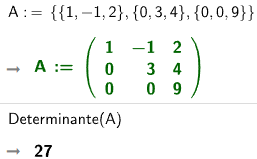
\includegraphics[width=150pt,height=120pt]{img/imagen16.png}
    \caption{Determinante de la matriz A en GeoGebra}
\end{figure}

\begin{center}
    \textit{\textbf{Solución: }Debido a que el determinante de la matriz A es diferente de cero, es decir, que es linealmente independiente, entonces se puede decir que sí genera el espacio $\mathbb{R}^3$.}
\end{center}

\begin{figure}[ht!]
    \centering
    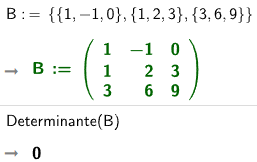
\includegraphics[width=150pt,height=120pt]{img/imagen17.png}
    \caption{Determinante de la matriz A en GeoGebra}
\end{figure}

\begin{center}
    \textit{\textbf{Solución: }Debido a que el determinante de la matriz B es igual a cero, es decir, que es linealmente dependiente, entonces se puede decir que no genera el espacio $\mathbb{R}^3$.}
\end{center}
